\documentclass[a4paper]{article}

\usepackage[pdftex]{graphicx}
\usepackage[margin=3cm]{geometry}
\usepackage{verbatim,moreverb,amssymb,amsmath}


\newcounter{question}
\newcommand{\question}[1]{\refstepcounter{question}\section*{Question~\thequestion~~~\small\emph{(#1)}}}
\renewcommand*\thequestion{\arabic{question}}


\begin{document}

\pagestyle{empty}
\thispagestyle{empty}



\noindent
\begin{minipage}{\columnwidth}
  \centering
  \Large
  DA4002 (HT11) Halmstad University\\
  Introduction to Algorithms, Data Structures, and Problem Solving\\[3\baselineskip]
  \Huge
  Written Exam\\
  \Large
  Tuesday, October 30, 2012\\[2\baselineskip]
  Examiner: Roland Philippsen
\end{minipage}

\vfill

\noindent
\begin{center}
\fbox{
  \begin{minipage}{0.8\columnwidth}
    \textbf{Student Name:}\\[3\baselineskip]
  \end{minipage}
}
\end{center}

\vfill



\section*{Rules}

Aside from the obvious rules of conduct exams (e.g.\ no chatting):

\begin{itemize}
\item
  \textbf{No computing devices} (laptops, phones, calculators, \emph{etc}).
\item
  \textbf{No books or printouts} except for non-electronic dictionaries.
\item
  \textbf{Allowed hand-written notes}: two sheets of A4 paper (front and back).
\end{itemize}



\section*{General Guidelines}

\begin{itemize}
\item
  \textbf{Read carefully} and pace yourself.
  You can solve the problems in any order you want, but later problems may be easier to solve after you have answered the preceding questions.
\item
  \textbf{Write clearly} and draw clear diagrams.
  If you need to correct a mistake, then cleanly cross out the wrong answer and clearly indicate where the correction can be found.
\item
  \textbf{Indicate the question number} for each of your answers.
  If a question has sub-questions, indicate the sub-question number after the main question number, separated by a dot.
  For example, question 3 has 4 sub-questions, and their answers should be numbered 3.1, 3.2, 3.3, and 3.4.
\end{itemize}



\pagebreak
\pagestyle{plain}
\thispagestyle{plain}
\setcounter{page}{1}



\question{3 points}

Below are three diagrams \textbf{(1)}, \textbf{(2)}, and \textbf{(3)}.
Each of them shows the result of inserting the values $\{5, -2, -3, 1, 9, 6\}$ into a different type of data structure.
To the right of the diagrams are three data structure declarations \textbf{(A)}, \textbf{(B)}, and \textbf{(C)}.
Each of them corresponds to one of the diagrams.
On the next page, there are three implementations of an \textbf{\texttt{insert}} function.
They are labelled \textbf{(D)}, \textbf{(E)}, and \textbf{(F)}.
Each implementation is for a different type of data structure.

\vfill

\noindent
Fill in the table at the bottom of this page.
For each of the diagrams
\begin{enumerate}
\item
  choose the corresponding declaration (from this page),
\item
  choose the corresponding implementation (from the next page),
\item
  and write down the name of the data structure.
\end{enumerate}

\vfill

\noindent
\begin{minipage}{0.4\columnwidth}
  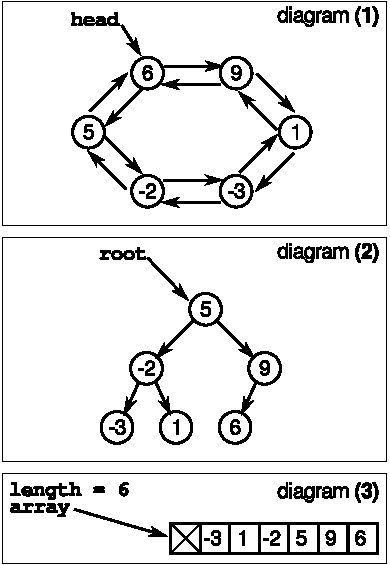
\includegraphics[width=\columnwidth]{q1.pdf}
\end{minipage}\hfill
\begin{minipage}{0.5\columnwidth}
  \small
  \fbox{%
    \begin{minipage}{\columnwidth}
      \hfill declaration \textbf{(A)}
      \verbatimtabinput{clist-decl.txt}
  \end{minipage}}
  \fbox{%
    \begin{minipage}{\columnwidth}
      \hfill declaration \textbf{(B)}
      \verbatimtabinput{minheap-decl.txt}
  \end{minipage}}
  \fbox{%
    \begin{minipage}{\columnwidth}
      \hfill declaration \textbf{(C)}
      \verbatimtabinput{bstree-decl.txt}
  \end{minipage}}
\end{minipage}

\vfill

\begin{center}
  \begin{tabular}{|c|p{0.2\columnwidth}|p{0.2\columnwidth}|p{0.5\columnwidth}|}
    \hline
            & declaration  & implementation & \\
    diagram & (A, B, or C) & (D, E, or F)   & data structure name \\
    \hline
    &&&\\
    \textbf{(1)} & & & \\
    &&&\\
    \hline
    &&&\\
    \textbf{(2)} & & & \\
    &&&\\
    \hline
    &&&\\
    \textbf{(3)} & & & \\
    &&&\\
    \hline
  \end{tabular}
\end{center}


\clearpage

\subsection*{Implementations for Question 1}

\noindent
\fbox{%
  \begin{minipage}{\columnwidth}
    \hfill implementation \textbf{(D)}
    \footnotesize
    \verbatimtabinput{minheap-insert.txt}
\end{minipage}}

\vfill

\noindent
\fbox{%
  \begin{minipage}{\columnwidth}
    \hfill implementation \textbf{(E)}
    \footnotesize
    \verbatimtabinput{bstree-insert.txt}
\end{minipage}}

\vfill

\noindent
\fbox{%
  \begin{minipage}{\columnwidth}
    \hfill implementation \textbf{(F)}
    \footnotesize
    \verbatimtabinput{clist-insert.txt}
\end{minipage}}

\clearpage


\question{3 points}

For each of the implementations \textbf{(D)}, \textbf{(E)}, and \textbf{(F)} from Question~1,
write a procedure that iterates over all the items in the corresponding data structure and prints the values that they store.
The order in which the items are printed does not matter.
You can use pseudo-code or C.


\clearpage


\question{4 points}

In a \emph{multilist}, items have multiple link fields and belong to more than one list at the same time.
For example, points can be stored such their order along X and Y is maintained independently.
In this case, there is one link field (pointer) for the next item along X, and one for the next item along Y.
There also are two separate heads, because the start of the list that is sorted along X will usually be different from the start of the list that is sorted along Y.

The diagram below shows five points labeled \textbf{A}, \textbf{B}, \textbf{C}, \textbf{D}, and \textbf{E}.
Each has different X and Y coordinates, written in parentheses after the label.

\vfill

\noindent
\begin{center}
  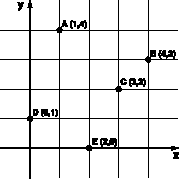
\includegraphics[width=0.4\columnwidth]{q2a.pdf}
\end{center}

\vfill

\begin{enumerate}
\item
  At the bottom of this page is an incomplete diagram for a \emph{multilist} as described above.
  
  Your first task is to fill in and connect the \texttt{Point} boxes:
  write one of the labels (A, B, C, D, and E) into each box, and draw arrows from the \texttt{xnext} fields.
  Also draw an arrow from \texttt{xhead} to the appropriate start box.
  Then, do the same for the Y coordinate, by adding arrows for the \texttt{ynext} and \texttt{yhead} pointers.
  
  Verify your work by checking that:
  \begin{itemize}
  \item
    When you start at \texttt{xhead} and repeatedly follow the \texttt{xnext} link, you visit all points by increasing X coordinate.
  \item
    Likewise, when you start at \texttt{yhead} and follow the \texttt{ynext} links, the points are visited by increasing Y coordinate.
  \end{itemize}
  
\item
  Using pseudo-code or C, write a procedure to insert a point into such a sorted multilist.
  Points are specified using their X and Y coordinates.
  You have to provide a declaration for the data structure along with your procedure.
  Take care to properly handle the initial case of inserting into an empty list.
\end{enumerate}

\vfill

\noindent
\begin{center}
  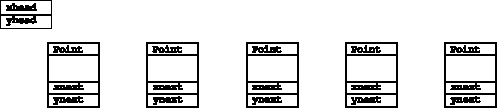
\includegraphics[width=\columnwidth]{q2b.pdf}
\end{center}


\clearpage

\question{6 points}

\begin{enumerate}

\item
  The execution time $T_A$ of program $A$ has been measured on a problem of size $N=1024$:
  it took $T_A(N) = 640ms$ to run.
  What is the expected execution time $T'_A$ for a problem of size $N'=128$, if $A$'s big-Oh complexity is\\
  \emph{(i)} logarithmic: $T_A(N) \in O(\log N)$ ?\\
  \emph{(ii)} square: $T_A(N) \in O(N^2)$ ?
  
  \emph{\textbf{Notice the table of numeric values} for $x^2$, $x^3$, and $2^x$ on the bottom of this page, to help you with the computations.}
  
\item
  Program $B$ required $T_B=10ms$ to run on a problem of size $N=1000$.
  What problem size $N'$ can be expected to complete, if the available time is $T'_B=270ms$ and the big-Oh complexity of $B$ is\\
  \emph{(i)} linear: $T_B(N) \in O(N)$ ?\\
  \emph{(ii)} cubic: $T_B(N) \in O(N^3)$ ?
  
\item
  The time $T_C$ it takes to run \texttt{function\_C} for $N=512$ is $T_C=5ms$.
  Based on a big-Oh complexity analysis of the code shown below, how much time will it take for $N'=2048$?
  You can assume that the various \texttt{slow\_X} functions take significantly longer to execute than any of the other operations.
  
\item
  The time $T_D$ taken by \texttt{function\_D} given below is $30ms$ for an array of length $N=512$.
  How large of an array can be handled when we only have $10ms$ available?
  Again, you can assume that the \texttt{slow\_5} function takes up the majority of the computation time.
  
\end{enumerate}
  
\vfill

\noindent
\fbox{%
  \begin{minipage}[t]{0.40\columnwidth}
    \small
    \verbatimtabinput{q3a.txt}
\end{minipage}}\hfill
\fbox{%
  \begin{minipage}[t]{0.56\columnwidth}
    \small
    \verbatimtabinput{q3b.txt}
\end{minipage}}

\vfill

\noindent
\begin{tabular}{|l|r|r|r|r|r|r|r|r|r|r|r|r|r|r|r|}
  \hline
  $x=$   & 0 & 1 & 2 &  3 &  4 &   5 &   6 &   7 &   8 &   9 &   10 &   11 &   12 &   13 &    14 \\
  $x^2=$ & 0 & 1 & 4 &  9 & 16 &  25 &  36 &  49 &  64 &  81 &  100 &  121 &  144 &  169 &   196 \\
  $x^3=$ & 0 & 1 & 8 & 27 & 64 & 125 & 216 & 343 & 512 & 729 & 1000 & 1331 & 1728 & 2197 &  2744 \\
  $2^x=$ & 1 & 2 & 4 &  8 & 16 &  32 &  64 & 128 & 256 & 512 & 1024 & 2048 & 4096 & 8192 & 16384 \\
  \hline
\end{tabular}


\clearpage

\question{5 points}

The Needleman-Wunsch algorithm, which has been studied in detail during project~2, can be used to align different kinds of sequences.
For colors, the match score can measure how similar one color is to the others.
This can be expressed in a lookup table (you could also call it a similarity matrix).
For example, assume the following color symbols and match scores:

\begin{center}
  \begin{minipage}{0.5\columnwidth}
    color similarity \emph{(match scores)}\\
    \begin{tabular}{|c|cccccc|}
      \hline
      &  V &  B &  G &  Y &  O &  R \\
      \hline
      V & 10 &  2 & -3 & -6 & -3 &  2 \\
      B &  2 & 10 &  2 & -3 & -6 & -3 \\
      G & -3 &  2 & 10 &  2 & -3 & -6 \\
      Y & -6 & -3 &  2 & 10 &  2 & -3 \\
      O & -3 & -6 & -3 &  2 & 10 &  2 \\
      R &  2 & -3 & -6 & -3 &  2 & 10 \\
      \hline
    \end{tabular}\\
    \textbf{gap cost}: -3
  \end{minipage}
  \begin{minipage}{0.3\columnwidth}
    \noindent
    \textbf{V} stands for \emph{violet}\\
    \textbf{B} stands for \emph{blue}\\
    \textbf{G} stands for \emph{green}\\
    \textbf{Y} stands for \emph{yellow}\\
    \textbf{O} stands for \emph{orange}\\
    \textbf{R} stands for \emph{red}
  \end{minipage}
\end{center}

\vspace{2\baselineskip}

\noindent
You are asked to \textbf{align the sequences VBR and YOG}.

\begin{enumerate}
\item
  Given the above definitions, create and fill the cost propagation table used by the Needleman-Wunsch algorithm.
\item
  What is the optimal alignment score between these two sequences?
\item
  What are the optimal alignments?
  Note that there is more than one solution.
\end{enumerate}

\clearpage


\question{4 points}

\begin{enumerate}
  
\item
  There is a bug in the following implementation of insertion sort.
  For example, if it is given an array that contains the numbers $\{ 6, 0, 7, 3, 8, 5, 1, 4, 9, 2 \}$, it will produce the incorrect $\{ 6, 6, 7, 7, 8, 8, 8, 8, 9, 9 \}$.
  What is wrong, and how can it be fixed?
  
  \begin{center}
    \fbox{%
      \begin{minipage}{0.7\columnwidth}
        \small
        \verbatimtabinput{isort-buggy.txt}
    \end{minipage}}
  \end{center}
  
\item
  For removing the topmost item of a min-heap, we overwrite \texttt{array[1]} with the last item, shrink the array, and then call \texttt{bubble\_down} in order to restore the min-heap property.
  However, the following implementation of bubble-down contains a mistake.
  For example, after successfully inserting the numbers $\{ 1, 2, 3, 1, 2, 5, 4, 3 \}$ onto the heap, the produced incorrect order of removal is $\{ 1, 3, 4, 5, 2, 2, 3, 1 \}$.
  What is wrong, and how can it be fixed?
  
  \begin{center}
    \fbox{%
      \begin{minipage}{0.7\columnwidth}
        \small
        \verbatimtabinput{bdown-buggy.txt}
    \end{minipage}}
  \end{center}

\end{enumerate}

\end{document}
